\chapter{System overview}
\label{ch:sysOverview}
This chapter provides an overview of the VINS-Mono SLAM system proposed by  
\citep{Qin2017VINS} as visualized in \autoref{fig:VINSsys}. The focus lies on 
the parts of the system which are crucial for this work whereas the rest is 
only described briefly. For a detailed description of the system we refer to 
\citep{Qin2017VINS}.

\begin{figure}[h!]
  \centering
  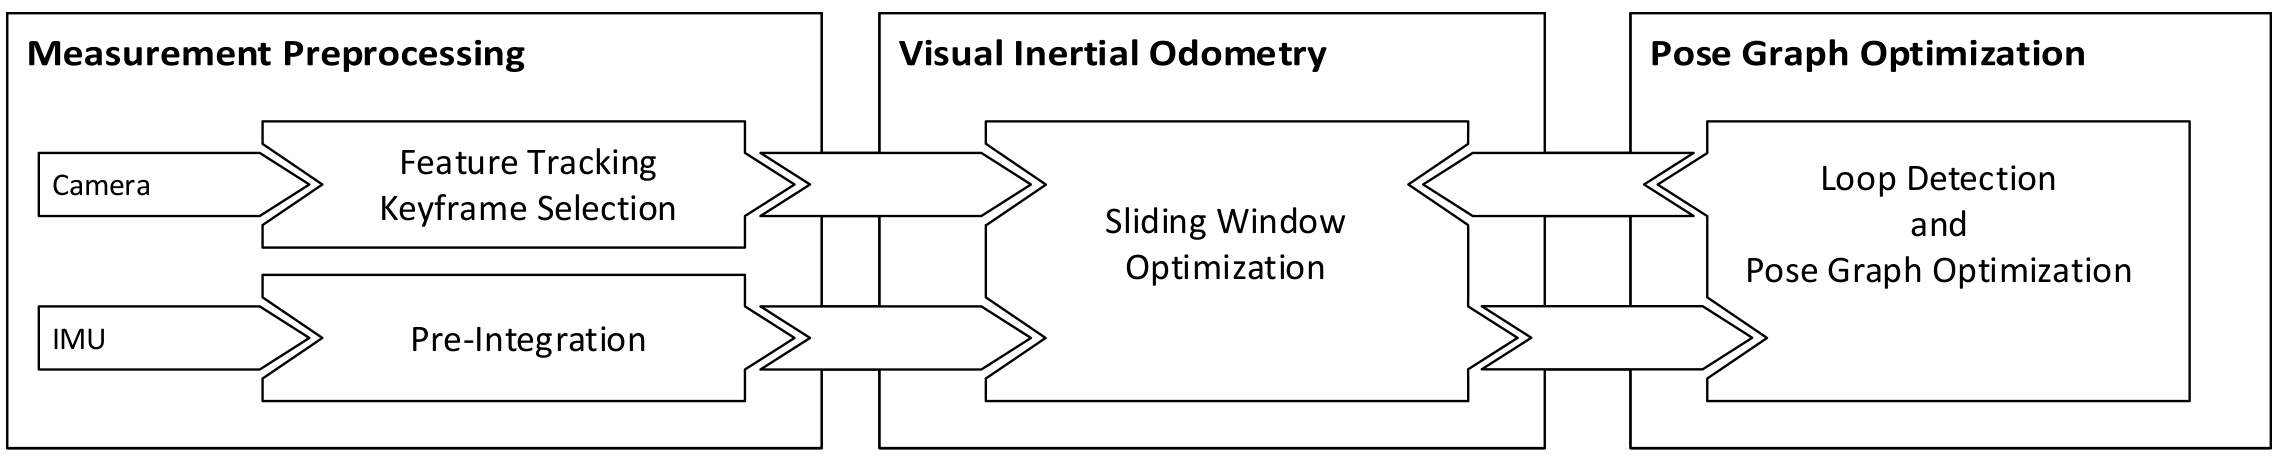
\includegraphics[width=1\textwidth]{images/system.png}
  \caption{VINS-Mono SLAM system overview. Shown are the preprocessing module 
on the left side, the front-end in the middle and the back-end on the right 
side.}
  \label{fig:VINSsys}
\end{figure}

\section{Measurement Preprocessing}
\label{sec:measPreprocess}
In the preprocessing step (left side in \autoref{fig:VINSsys}), features 
in the frames are extracted and tracked 
over consecutive frames using the KLT sparse optical flow algorithm 
\cite{lucas1981}. To maintain a minimum number of features in each image, 
additional corner features are detected. Keyframes are also selected in the 
preprocessing step. The current frame is selected as keyframe if one of the 
following two criteria is fulfilled: 
\begin{enumerate}
  \item The average parallax apart from the previous keyframe is beyond a certain threshold.
  \item The number of tracked features goes below a certain threshold.
\end{enumerate}

The \ac{IMU} measurements between two consecutive frames are pre-integrated  
including bias correction as proposed in \citep{Forster2017Manifold}. 

\section{Visual Inertial Odometry}
For a robust and accurate state estimation a tightly-coupled monocular \ac{VIO} 
pipeline is used (middle part in \autoref{fig:VINSsys}). It performs a 
non-linear \ac{BA} optimization followed by a marginalization.

\subsection{Optimization}
\label{subsec:optimization}
In order to bound the computational complexity, the optimization is performed 
in a sliding window manner. The optimization is a visual-inertial \ac{BA}. The 
sum of prior and the Mahalonobis norm of all measurement residuals is minimized 
over the full state vector $\mathbfcal{X}$ to obtain a maximum posteriori 
estimation: 

\begin{equation}\label{eq:optimization}
\displaystyle
\min_{\mathbfcal{X}} \left\{ \left\lVert \vec{r}_p - \vec{H}_p\mathbfcal{X} 
\right\rVert^{2} +
\sum_{k\in \mathcal{B}} \left\lVert 
\vec{r}_\mathcal{B}\left(\vhat{z}^{b{_k}}_{b_{k\!+\!1}}, \mathbfcal{X} 
\right)\right\rVert^{2}_{\vec{P}^{b_k}_{b_{k\!+\!1}}} + 
\sum_{\left(l,j\right) \in \mathcal{C}} \rho \left( \left\lVert 
\vec{r}_\mathcal{C}\left(\vhat{z}^{c_{j}}_{l_{\textcolor{white}{+}}}, 
\mathbfcal{X} \right)\right\rVert^{2}_{\vec{P}^{c_j}_{l}} \right)
\right\},
\end{equation}
where $\rho$ is the Huber norm. 
$\vec{r}_\mathcal{B}\left(\vhat{z}^{b{_k}}_{b_{k\!+\!1}}, \mathbfcal{X} 
\right)$
and 
$\vec{r}_\mathcal{C}\left(\vhat{z}^{c_{j}}_{l_{\textcolor{white}{+}}}, 
\mathbfcal{X} \right)$
are the residuals for the \ac{IMU} and the visual measurements, respectively. 
The \ac{IMU} residual consists of constraints on the poses, the velocity, and 
the orientation of the \ac{IMU} between two consecutive (key-)frames in the 
sliding window. The \ac{IMU} residual also contains the acceleration and 
gyroscope bias. The visual measurement residual consist of constraints on the 
poses and the orientation of the (key-)frames and the features observed in these 
frames. A detailed description of the residuals can be found in 
\citep{Qin2017VINS}. $\{ \vec{r}_p, \vec{H}_p\}$ is the prior information 
retrieved from the marginalization described in 
\autoref{subsec:marginalization}. It contains constraints on the pre-integrated 
\ac{IMU} factor between the marginalized and the subsequent keyframe and on the 
features observed in the marginalized keyframe. \\

The \ac{BA} optimization is performed over a sliding window, containing the 
latest two frames, a new arriving frame, and the eight previous 
keyframes. An illustration of the sliding window is shown in 
\autoref{fig:slideWindow}, with the corresponding graph representation in 
\autoref{fig:slideWindowGraph_a}.

\begin{figure}[h!]
  \centering
      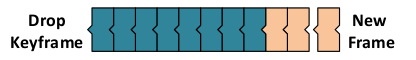
\includegraphics[width=1\textwidth]{images/slideWindow.png}
  \caption{Representation of the sliding window. The eight previous keyframes 
are marked in blue with the oldest one most left. The latest two frames in the 
window and a new arriving frame, illustrated on the right most side, are marked 
in orange.}
  \label{fig:slideWindow}
\end{figure}

\begin{figure}[h!]
\begin{minipage}[b]{1\linewidth}
\centering\large 
  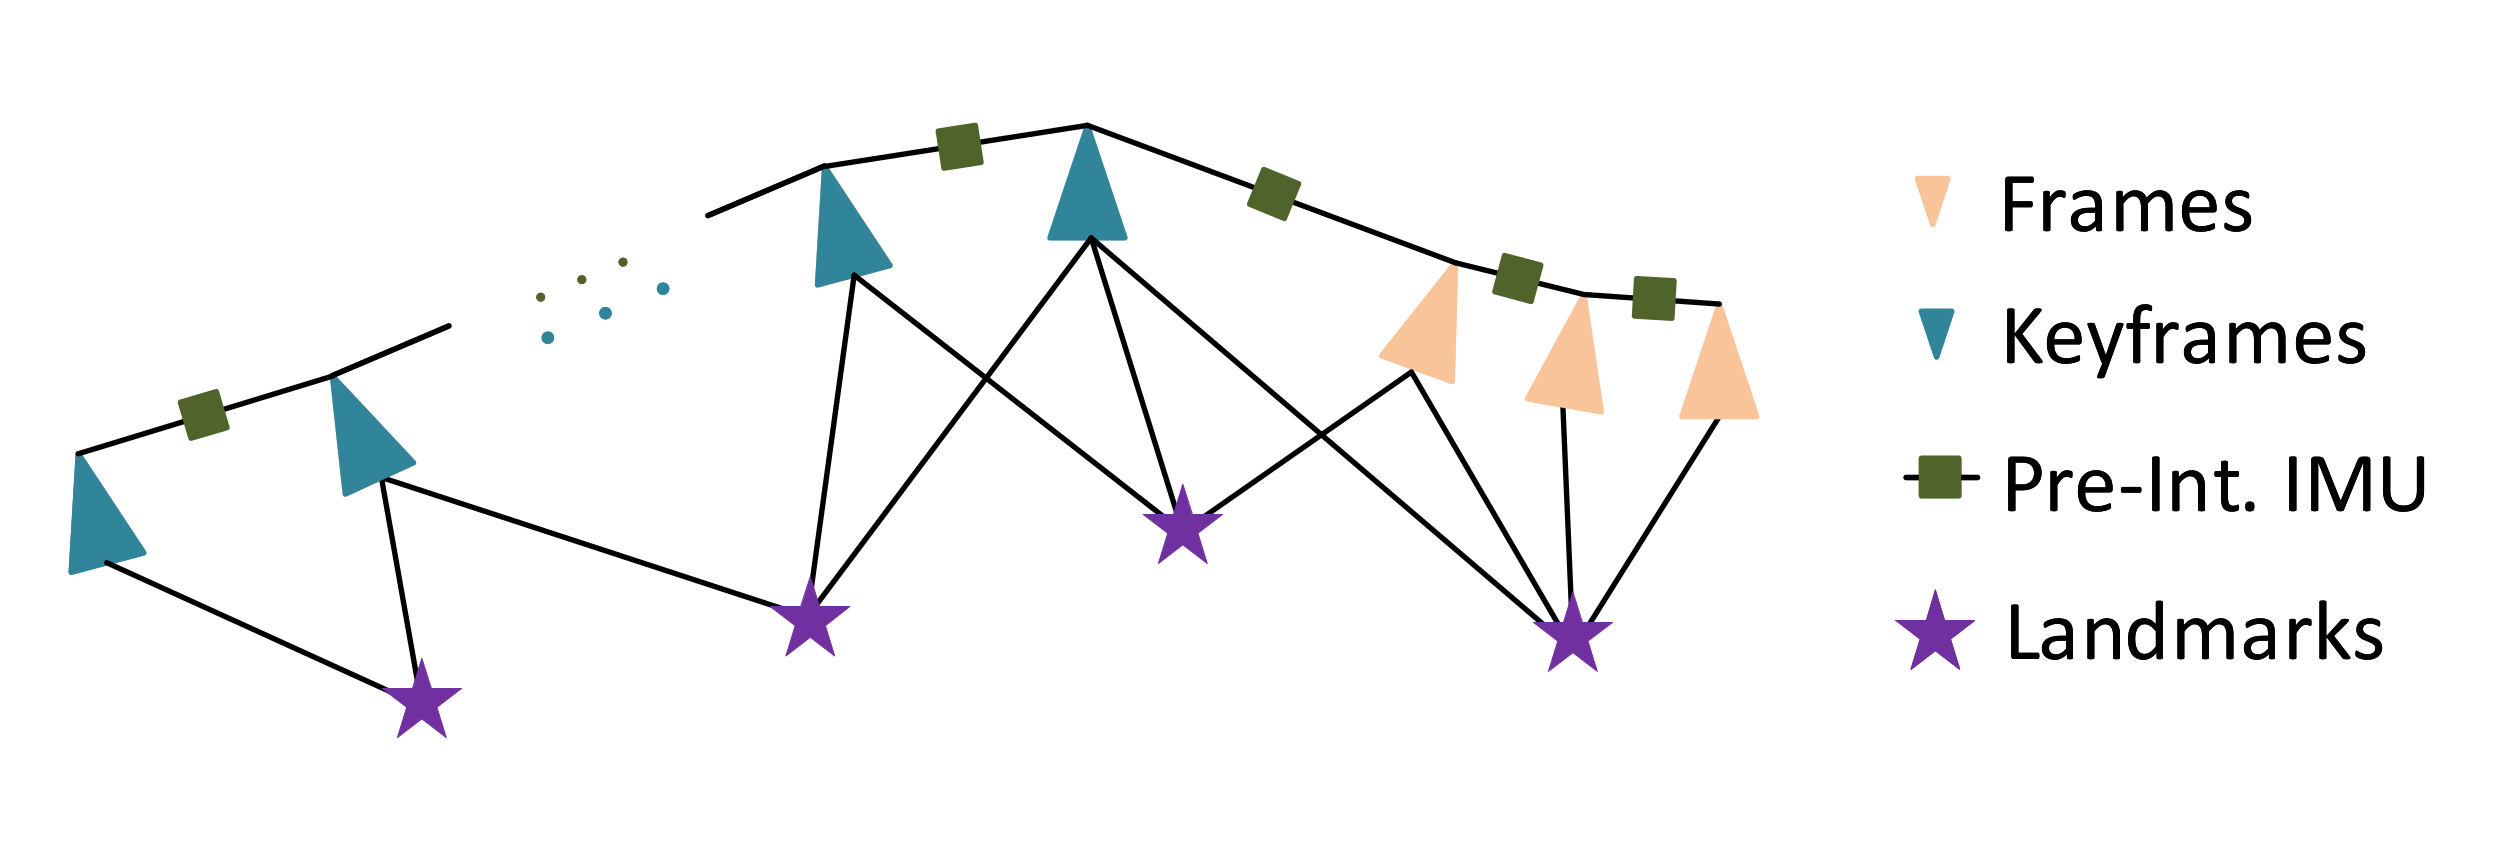
\includegraphics[width=1\textwidth]{images/throw_1.png}
\subcaption{Graph of the state variables and measurements the \ac{BA} 
optimization is performed on.}
\label{fig:slideWindowGraph_a}

\centering\large 
  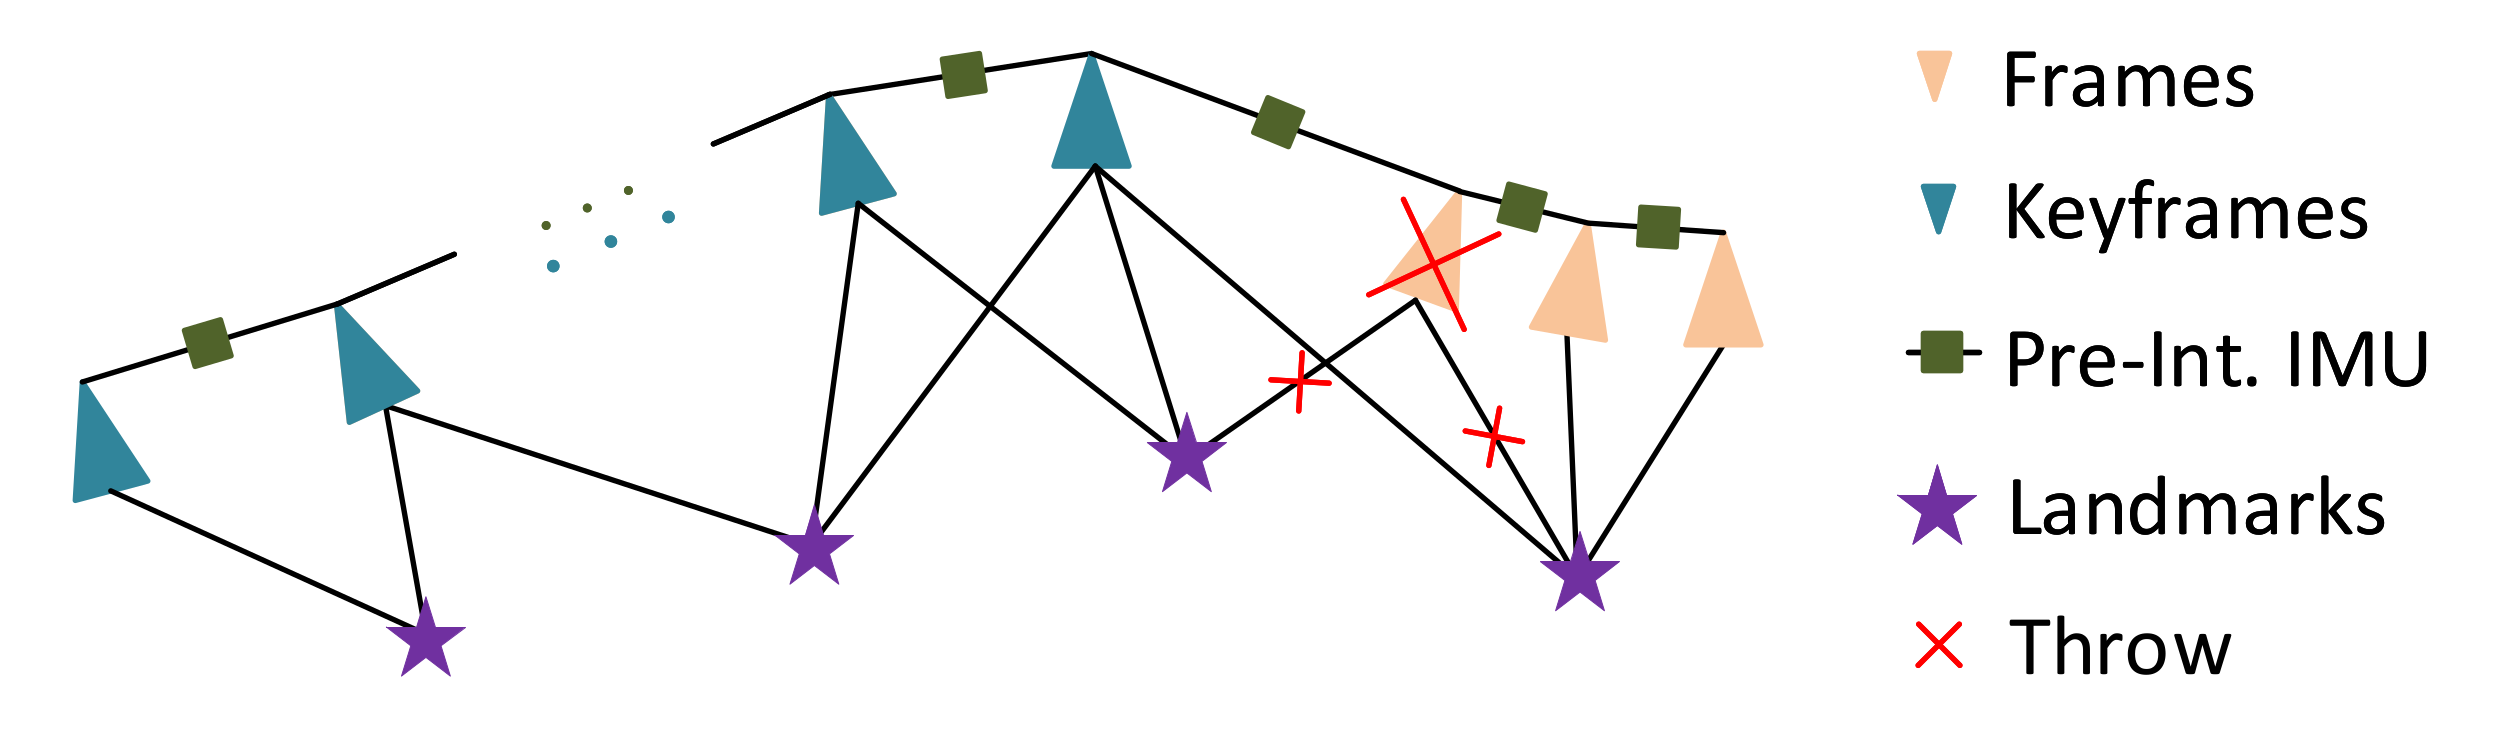
\includegraphics[width=1\textwidth]{images/throw_2.png}
\subcaption{Graph of the state variables and measurements after the \ac{BA} 
optimization. If the second latest frame is not a keyframe, it is removed 
together with its corresponding visual measurements. The pre-integrated 
\ac{IMU} measurements are combined into one measurement·}
\label{fig:slideWindowGraph_b}

\centering\large 
  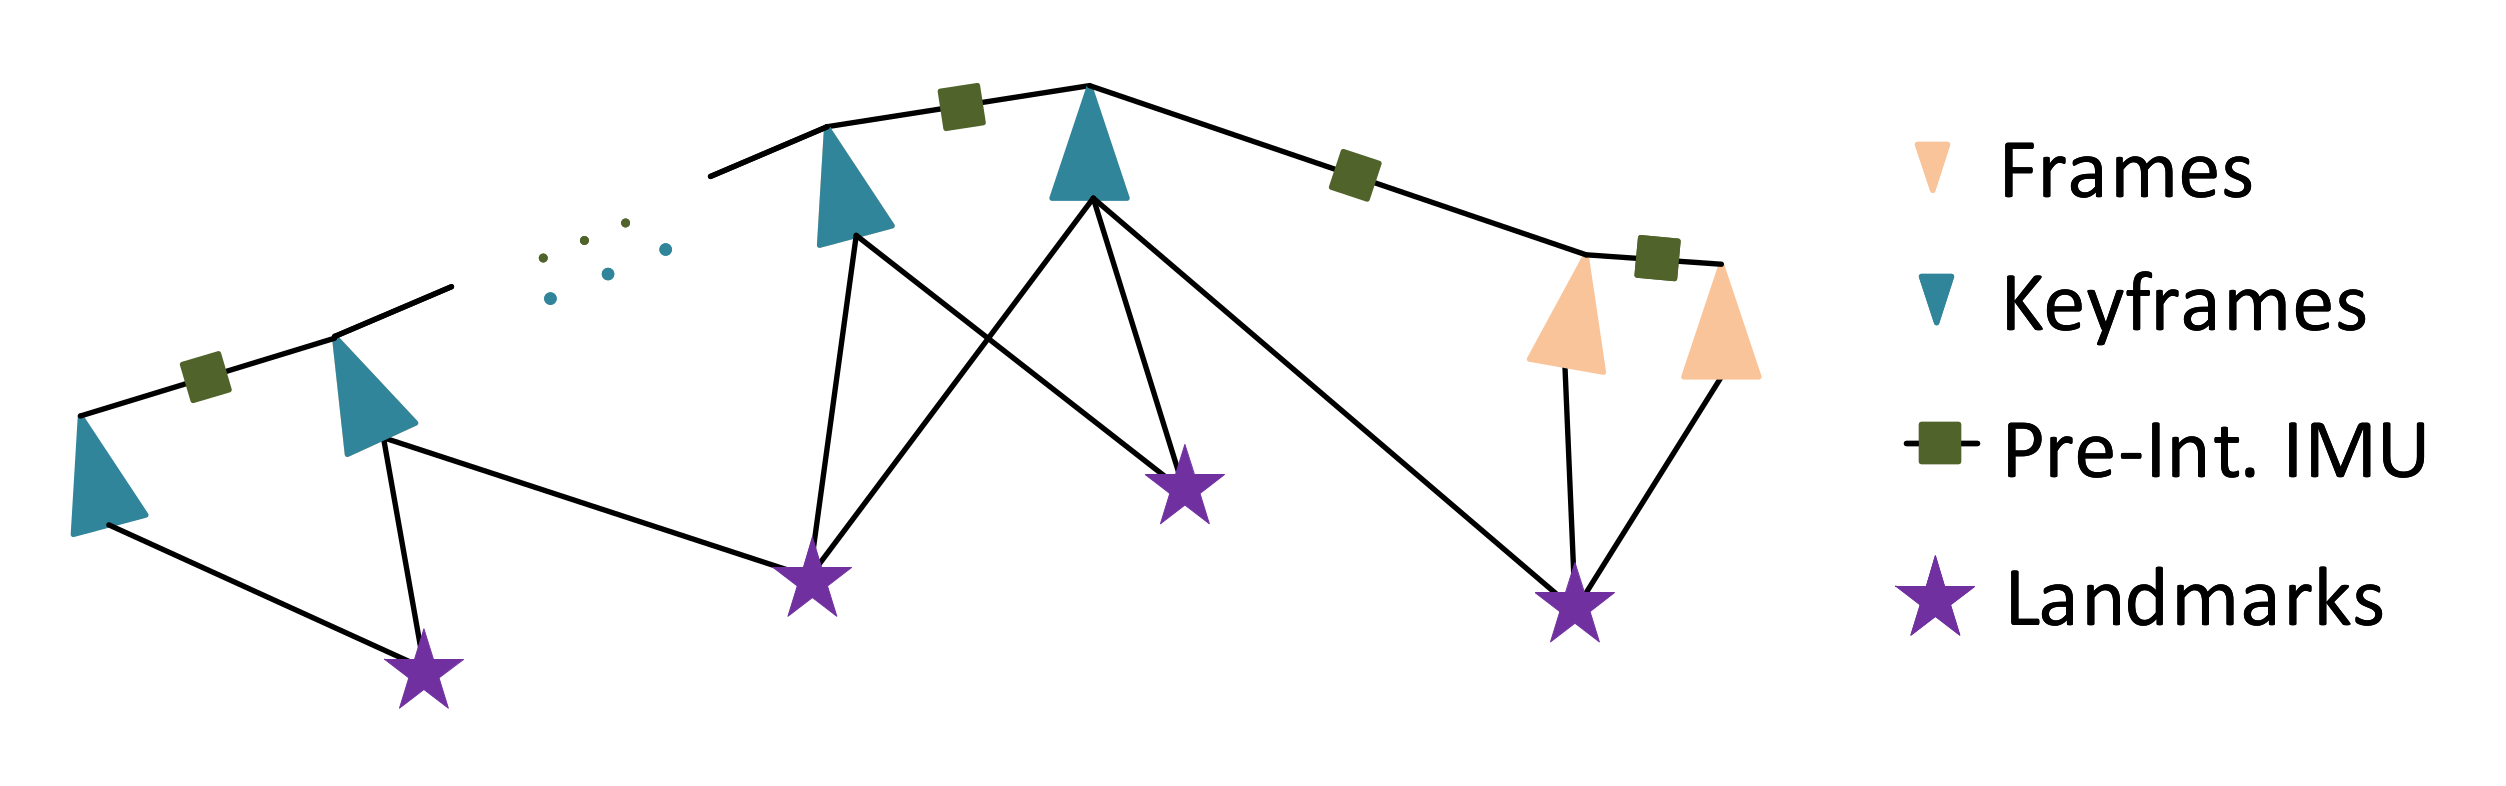
\includegraphics[width=1\textwidth]{images/throw_3.png}
\subcaption{Graph of the state variables and measurements, after the \ac{BA} 
optimization and marginalization, before a new frame arrives and the \ac{BA} 
optimization is performed.}
\label{fig:slideWindowGraph_c}
\end{minipage}%
  \caption{An illustration of the marginalization strategy 
(\subref{fig:slideWindowGraph_a})-(\subref{fig:slideWindowGraph_c}) if the
second latest frame is not a keyframe. Blue triangles mark the keyframe poses 
and orange triangles mark the latest two frame poses and the pose of the new 
arriving frame. The stars represent landmarks that are observed within the 
(key-)frames. The green squares represent the pre-integrated \ac{IMU} 
measurements.}
  \label{fig:slideWindowGraph}
\end{figure}

% With $\mathcal{B}$ beeing the set of all \ac{IMU} measurements and $\mathcal{C}$ the set of all features which have been observed at least twice in the current sliding window. To limit the effect of outliers the visual measurements are $\{ \vec{r}_p, \vec{H}_p \}$ is the prior information retrieved from the marginalization.  


\subsection{Marginalization}
\label{subsec:marginalization}
There are two possible cases after the \ac{BA} optimization. If the second 
latest frame is not a keyframe, only the \ac{IMU} measurements are kept and the 
visual measurements are dropped, as shown in \autoref{fig:slideWindowGraph}. 
In case the second latest frame is a keyframe, it will stay in the window and 
the oldest keyframe is marginalized, as shown in \autoref{fig:marginalize}. The 
marginalization is performed in order to preserve constraints between the 
\ac{IMU} state and the features observed in the oldest keyframe. \\


\begin{figure}[h!]
\begin{minipage}[b]{1\linewidth}
\centering\large 
  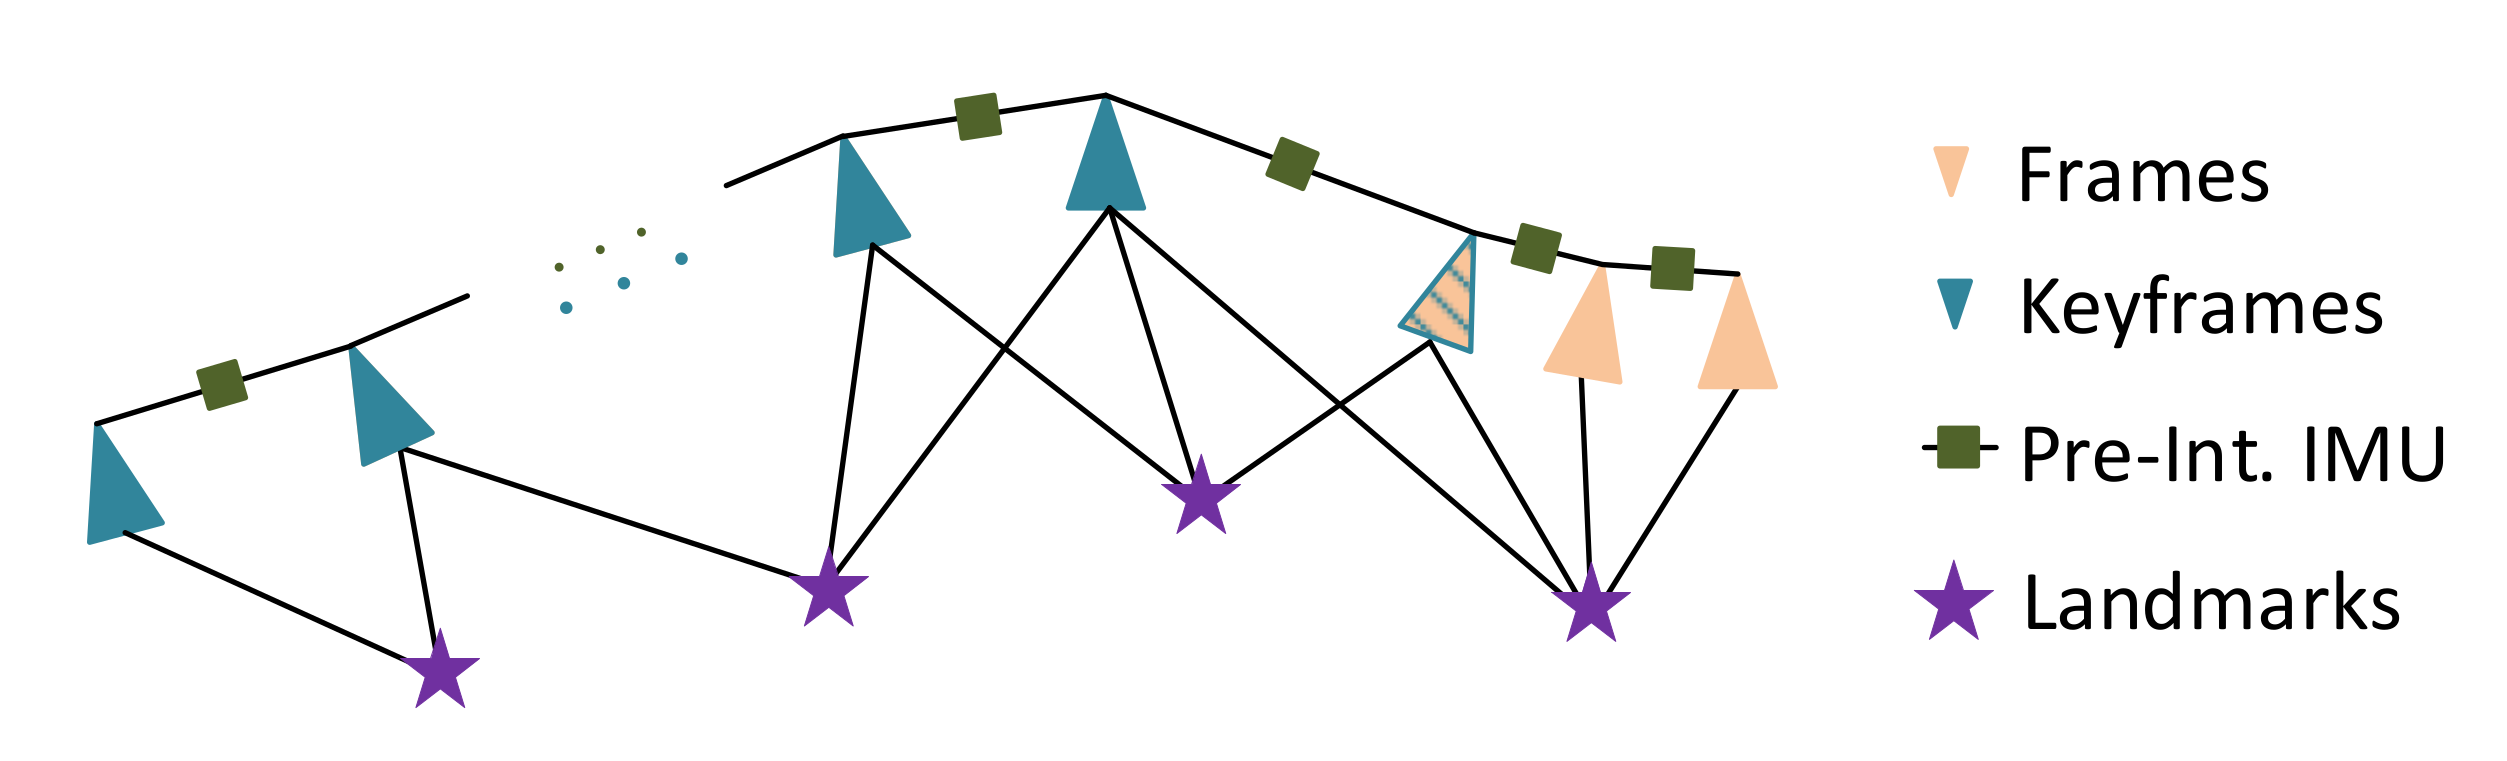
\includegraphics[width=1\textwidth]{images/marg_1.png}
\subcaption{Graph of the state variables and measurements the \ac{BA} 
optimization is performed on.}
\label{fig:marginalize_a}

\centering\large 
  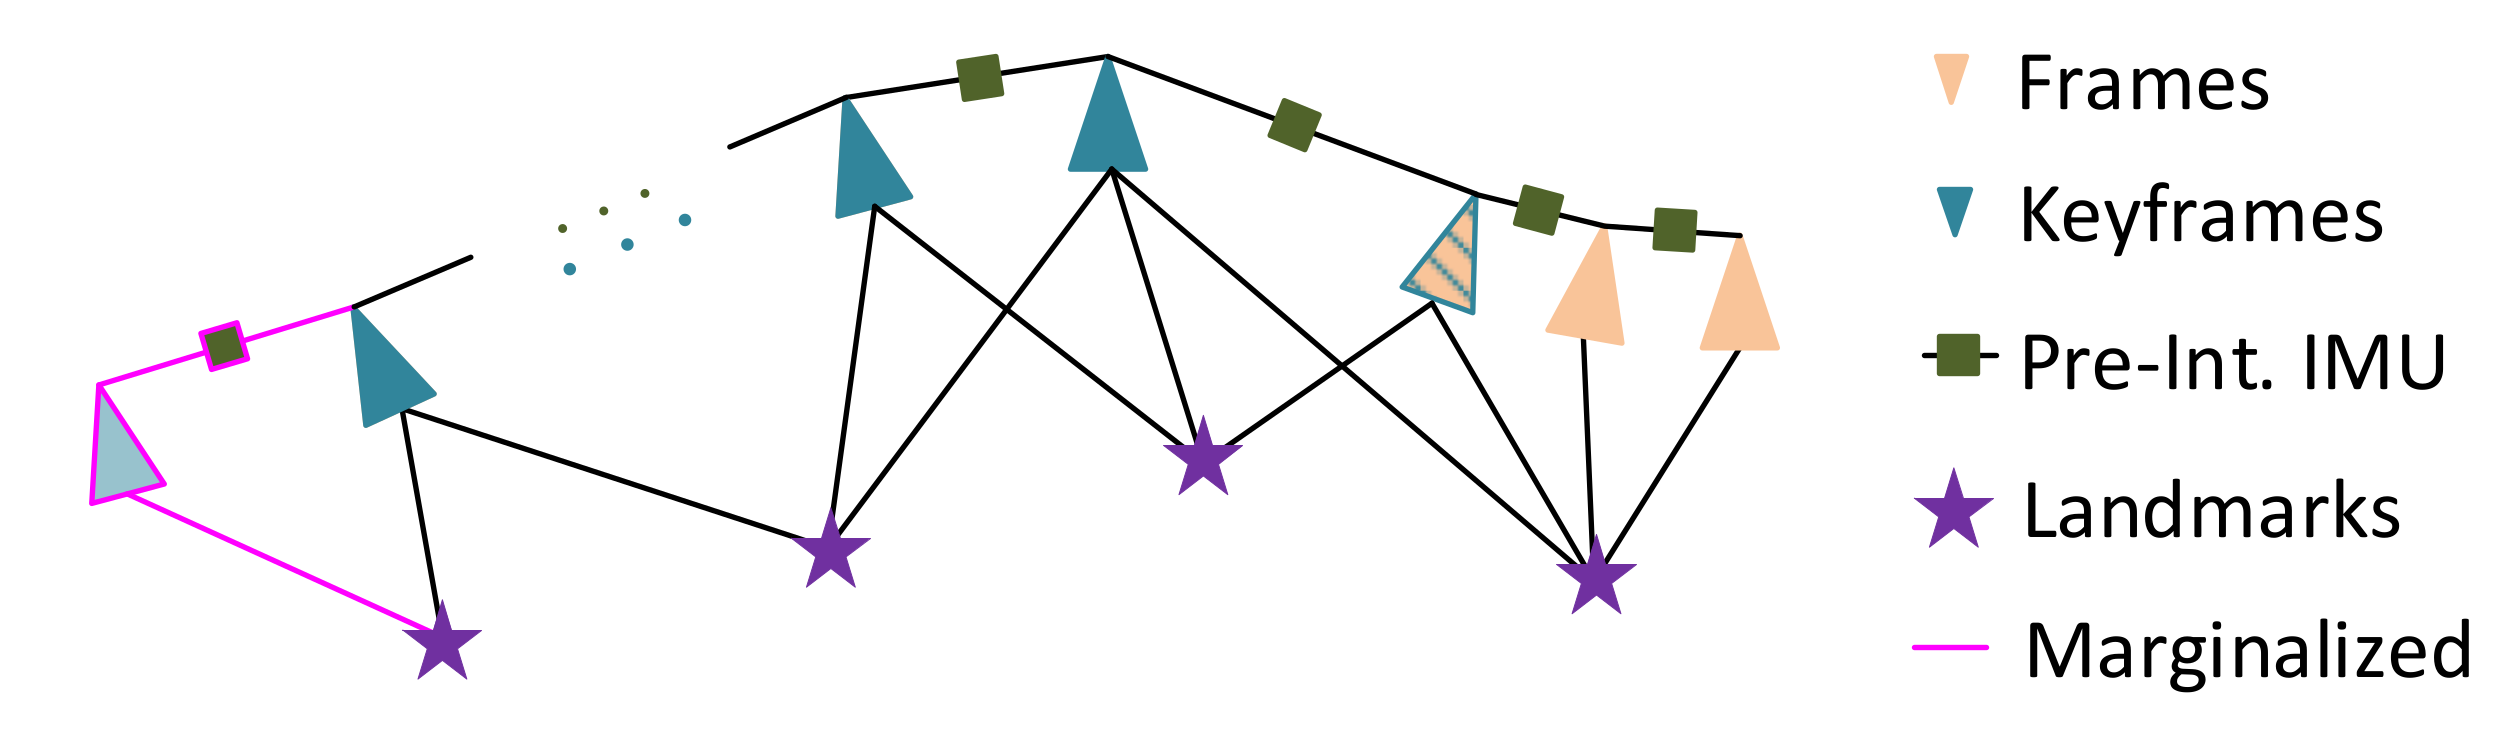
\includegraphics[width=1\textwidth]{images/marg_2.png}
\subcaption{Graph of the state variables and measurements after the \ac{BA} 
optimization. If the second latest frame is a keyframe, it is kept in the 
window, and the oldest keyframe and its corresponding visual and \ac{IMU} 
measurements are marginalized out. Marginalized measurements are turned into a 
prior.}
\label{fig:marginalize_b}

\centering\large 
  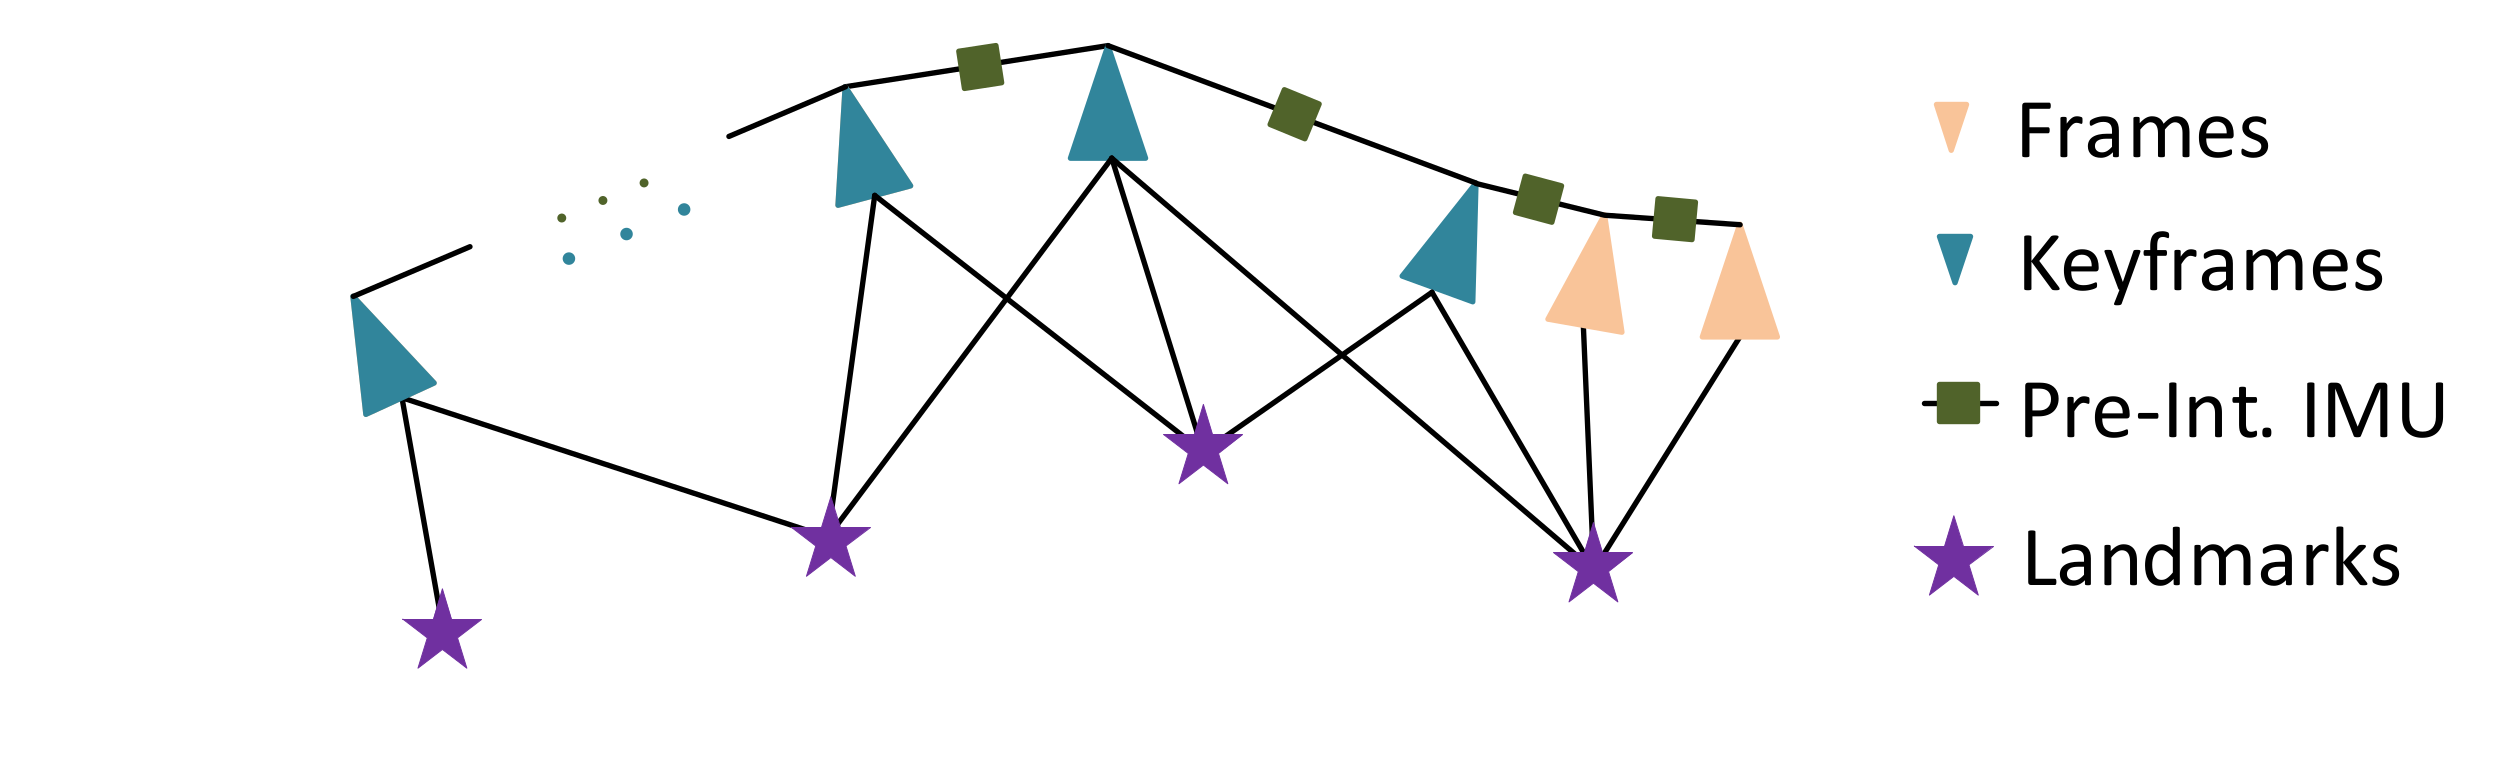
\includegraphics[width=1\textwidth]{images/marg_3.png}
\subcaption{Graph of the state variables and measurements, after the \ac{BA} 
optimization and marginalization, before a new frame arrives and the \ac{BA} 
optimization is performed.}
\label{fig:marginalize_c}
\end{minipage}%
  \caption{An illustration of the marginalization strategy 
(\subref{fig:marginalize_a})-(\subref{fig:marginalize_c})if the 
second latest frame is a keyframe. Blue triangles mark the keyframe poses and 
orange triangles mark the latest two frame poses and the pose of the new 
arriving frame. The stars represent landmarks that are observed within the 
(key-)frames. The green squares represent the pre-integrated \ac{IMU} 
measurements.}
  \label{fig:marginalize}
\end{figure}

The marginalization is carried out using the Schur complement 
\cite{sibley2010Slide}. A new prior related to the removed state is constructed 
and added to the existing prior in Equation \eqref{eq:optimization}.

\subsubsection{Schur Complement}
Marginalization out parameters of a linear system matrix is equivalent to 
applying 
the Schur complement on this linear system matrix, as explained in 
\citep{sibley2010Slide}. For example, given the system
\begin{equation}\label{eq:schur_system}
  \begin{bmatrix}
    \vec{\Lambda}_a & \vec{\Lambda}_{b} \\
    \vec{\Lambda}_b^\top & \vec{\Lambda}_c
  \end{bmatrix} 
  \begin{bmatrix}
    \delta \vec{x}_a \\
    \delta \vec{x}_b
  \end{bmatrix} = 
  \begin{bmatrix}
    \vec{g}_a \\
    \vec{g}_b
  \end{bmatrix}.
\end{equation}
reducing the parameters $\vec{x}_a$ onto the parameters $\vec{x}_b$ leads to
\begin{equation}\label{eq:schur_complement}
  \begin{bmatrix}
    \vec{\Lambda}_a & \vec{\Lambda}_{b} \\
    0 & \vec{\Lambda}_c - \vec{\Lambda}_{b}^\top  \vec{\Lambda}_{a}^{-1} 
\vec{\Lambda}_{b}
  \end{bmatrix} 
  \begin{bmatrix}
    \delta \vec{x}_a \\
    \delta \vec{x}_b
  \end{bmatrix} = 
  \begin{bmatrix}
    \vec{g}_a \\
    \vec{g}_b -  \vec{\Lambda}_{b}^\top  \vec{\Lambda}_{a}^{-1} 
\vec{g}_{a}
  \end{bmatrix}.
\end{equation}
After this forward substitution step, the smaller lower-right system is 
independent of $\vec{x}_a$ and can be solved to update $\vec{x}_b$:
\begin{equation}\label{eq:schur_reduced}
\left[\vec{\Lambda}_c - \vec{\Lambda}_{b}^\top  \vec{\Lambda}_{a}^{-1} 
\vec{\Lambda}_{b} \right] \left[ \delta \vec{x}_b \right] = 
\left[ \vec{g}_b - \vec{\Lambda}_{b}^\top  \vec{\Lambda}_{a}^{-1} 
\vec{g}_a \right].
\end{equation}


In our case, the pose estimation problem can be described as a $2 \!\times \!2$ 
system of equations (for simplicity the \ac{IMU} states are included in the 
pose states):
\begin{equation}\label{eq:system}
  \begin{bmatrix}
    \vec{\Lambda}_m & \vec{\Lambda}_{mp} \\
    \vec{\Lambda}_{mp}^\top & \vec{\Lambda}_p
  \end{bmatrix} 
  \begin{bmatrix}
    \delta \vec{x}_m \\
    \delta \vec{x}_p
  \end{bmatrix} = 
  \begin{bmatrix}
    \vec{g}_m \\
    \vec{g}_p
  \end{bmatrix}.
\end{equation}
Where $\vec{x}_m$ and  $\vec{x}_p$ are composed of the observed 3D 
landmarks and the robot poses, respectively. The system matrix contains 
the ``pose block'' $\vec{\Lambda}_p$, the ``map block'' 
$\vec{\Lambda}_m$, and the ``observation block'' $\vec{\Lambda}_{mp}$. 
On the right-hand side of Equation \eqref{eq:system}, $\vec{g}_m$ and 
$\vec{g}_p$ are the vectors corresponding to the robot path and the map, 
respectively. \\

This system has the same structure as Equation \eqref{eq:schur_system} and 
therefore marginalization can be performed via Schur complement.


\section{Relocalization and Pose Graph Optimization}
The backend of the \ac{SLAM} system (right side in \autoref{fig:VINSsys})
consist of a loop closure and pose graph optimization. Thanks to the addition 
of \ac{IMU}, drift only occurs in 4 \ac{DoF} (the global 3D position $(x,y,z)$ 
and the rotation around the gravity direction), as described in 
\citep{Qin2017VINS}. To eliminate these drifts, VINS-Mono provides a 
tightly-coupled relocalization module which is seamlessly integrated with the 
monocular \ac{VIO}. \\

After relocalization, the local sliding window is aligned with the past poses. 
The pose graph optimization module uses these relocalization results 
to perform a 4 \ac{DoF} optimization to ensure the set of past poses is 
registered into a globally consistent configuration.
\\

In order to reduce the computational demand of the overall system, the 
loop closure and pose graph optimization is deactivated for this work.

\section{Implementation} \label{sec:implementation}
The optimization Equation \eqref{eq:optimization} is implemented using Google's 
\textit{ceres solver} \citep{ceres-solver}. The default settings regarding the 
parameters of the feature tracker and the optimization are the following:
\begin{itemize} 
 \item Maximum number of tracked features throughout the keyframes in the 
sliding window: 150 features.
 \item Maximum number of solver iterations: 8 iterations.
 \item Maximal solving time: 40 milliseconds.
\end{itemize}
The two break conditions of the optimization ensure real-time 
performance of the optimization step irrespective of 
convergence. However, the followed marginalization step is not guaranteed to be
performed before the next frame arrives, prohibiting real-time performance. 
Hence, if the overall optimization time (optimization and marginalization) 
between two consecutive frames has to be reduced, one needs to focus on the 
marginalization. 